%%%%%%%%%%%%%%%%%%%%%%% CHAPTER - 3 %%%%%%%%%%%%%%%%%%%%\\
\chapter{Methodology}
\label{C3} %%%%%%%%%%%%%%%%%%%%%%%%%%%%
\clearpage

This section outlines the proposed framework for document ranking using Retrieval-Augmented Generation (RAG) enhanced with Hypothetical Document Embedding (HyDE). The methodology integrates dense retrieval mechanisms with generative models to improve ranking accuracy and relevance. The system is designed to address key challenges in semantic understanding, contextual reasoning, and efficient ranking.

\subsection{System Architecture}
The proposed methodology consists of the following core components:
\begin{enumerate}
    \item \textbf{Query Preprocessing:} The input query is preprocessed to standardize its format and tokenize it for further processing.
    \item \textbf{Dense Retrieval:} Candidate documents are retrieved from a large corpus using dense embedding-based similarity search.
    \item \textbf{Hypothetical Embedding Generation (HyDE):} Hypothetical answers are generated for the query, which are encoded into embeddings for refined ranking.
    \item \textbf{Generative Reranking:} A large-scale language model scores and ranks the candidate documents by evaluating their relevance to both the query and the hypothetical embeddings.
    \item \textbf{Final Ranking:} The ranked list of documents is produced as the output.
\end{enumerate}

The overall workflow is illustrated in Fig.~\ref{fig:system_architecture}.

\begin{figure}[ht]
    \centering
    \begin{minipage}[t]{0.48\textwidth}
        \centering
        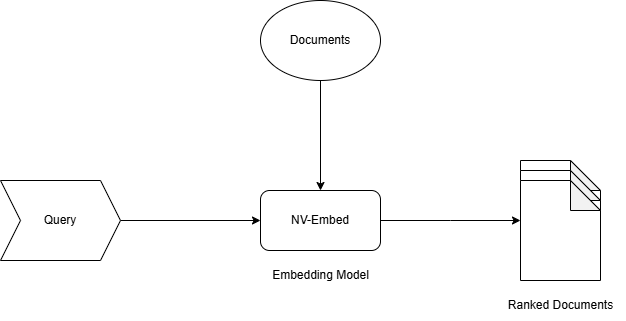
\includegraphics[width=\linewidth]{IMAGE/RAG_archi.png}
        \caption{Architecture 1: RAG}
        \label{fig:system_architecture}
    \end{minipage}
    \hfill
    \begin{minipage}[t]{0.48\textwidth}
        \centering
        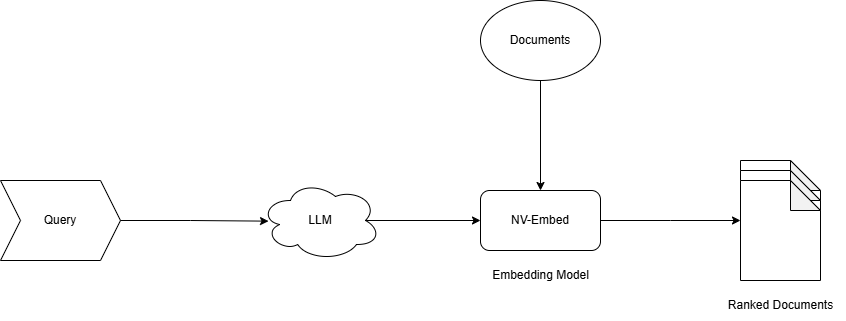
\includegraphics[width=\linewidth]{IMAGE/RAG_HyDE_archi.png}
        \caption{Architecture 2: HyDE}
        \label{fig:system_architecture}
    \end{minipage}
\end{figure}

\subsection{Dense Retrieval}
Dense retrieval forms the first stage of the pipeline, where the goal is to identify a subset of candidate documents from a large corpus that are semantically relevant to the input query. This is achieved using dense vector representations generated by transformer-based models such as BERT or DPR. The steps include:
\begin{enumerate}
    \item \textbf{Embedding Generation:} The input query and corpus documents are encoded into high-dimensional vectors using a pre-trained dense retriever.
    \item \textbf{Similarity Computation:} Cosine similarity is computed between the query vector and document vectors.
    \item \textbf{Top-K Retrieval:} The top-K documents with the highest similarity scores are retrieved for further processing.
\end{enumerate}

This stage ensures that only the most relevant documents are passed to the next phase, reducing computational overhead.

\subsection{Hypothetical Document Embedding (HyDE)}
The HyDE technique is incorporated to enhance the retrieval system by generating hypothetical answers to the query and utilizing these answers to refine the ranking. The steps involved are:
\begin{enumerate}
    \item \textbf{Hypothetical Answer Generation:} A generative model, such as Qwen2.5-3B-Instruct\cite{qwen2.5}, generates a hypothetical response to the input query. This response acts as a pseudo-query.
    \item \textbf{Embedding Creation:} Both the hypothetical answer and the candidate documents are encoded into dense vector embeddings.
    \item \textbf{Relevance Scoring:} Cosine similarity is computed between the embeddings of the hypothetical answer and the candidate documents. This generates an additional relevance score for each document.
\end{enumerate}

The HyDE component is particularly useful for addressing cases where the query is ambiguous or lacks sufficient context, as it hypothesizes missing information to improve document ranking.

\subsection{Generative Reranking}
In this stage, a large-scale generative language model is employed to score and rerank the documents based on their contextual relevance. The steps include:
\begin{enumerate}
    \item \textbf{Input Construction:} The retrieved documents and hypothetical embeddings are provided as input to the generative model along with the query.
    \item \textbf{Contextual Scoring:} The model generates a contextual score for each document by evaluating its relevance to the query and the hypothetical answer.
    \item \textbf{Ranking Adjustment:} The initial ranking is adjusted based on the contextual scores to produce the final ranked list.
\end{enumerate}

This step ensures that the ranking reflects not just surface-level similarity but also deeper semantic and contextual relevance.

\subsection{Implementation Details}
The proposed methodology was implemented using state-of-the-art tools and frameworks. Key details include:
\begin{itemize}
    \item \textbf{Dense Retriever:} The DPR (Dense Passage Retriever) model (NV-Embed-v2)\cite{nvembed} from Nvidia was used for encoding queries and documents.
    \item \textbf{Generative Model:} The Qwen2.5-3B-Instruct\cite{qwen2.5} model was utilized for hypothetical answer generation and generative reranking.
    \item \textbf{Embedding Framework:} The embeddings were normalized and processed using PyTorch\cite{pytorch} for efficient similarity computation.
    \item \textbf{Optimization:} Techniques such as batching and GPU acceleration were used to optimize performance on large datasets.
\end{itemize}

\subsection{Evaluation Pipeline}
The evaluation of the proposed methodology involves benchmarking its performance on standard dataset MS-MARCO\cite{DBLP:journals/corr/NguyenRSGTMD16} The evaluation metrics include:
\begin{itemize}
       \item \textbf{Accuracy:} This metric measures the proportion of correct predictions (both true positives and true negatives) among the total number of cases examined. It is calculated as:
    \begin{equation}
        \text{Accuracy} = \frac{\text{True Positives} + \text{True Negatives}}{\text{Total Number of Samples}}
    \end{equation}
    In our experiments, accuracy serves as a primary metric to evaluate the overall performance of the model across all classes.
        \item \textbf{Mean Reciprocal Rank (MRR):} Evaluates the ranking by considering the position of the first relevant document. For a set of queries Q, MRR is calculated as:
    \begin{equation}
        \text{MRR} = \frac{1}{|Q|} \sum_{i=1}^{|Q|} \frac{1}{\text{rank}_i}
    \end{equation}
    where $\text{rank}_i$ refers to the rank position of the first relevant document for the $i$-th query. MRR ranges from 0 to 1, with higher values indicating better ranking performance.
\end{itemize}

A detailed analysis of the results and comparisons with baseline methods is presented in Section~IV.

\subsection{Workflow Summary}
To summarize, the proposed methodology leverages dense retrieval, hypothetical embeddings, and generative reranking to achieve high-quality document rankings. By integrating these components into a unified pipeline, the system addresses key challenges in information retrieval and provides significant improvements in ranking accuracy and relevance.
